				\begin{figure}
					\begin{center}
						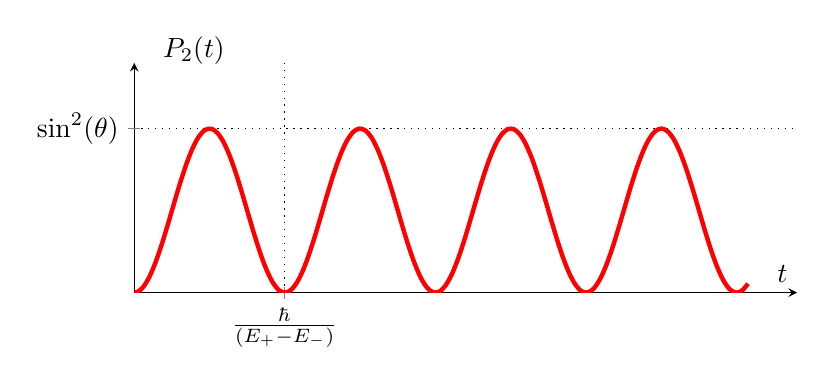
\begin{tikzpicture}
							\begin{axis}
							[
								axis x line=middle,
								axis y line=left,
								xmin = 0, xmax = {5.4},
								ymin = 0, ymax = {1.4},
								samples=200,
								xlabel=$t$,
								y label style={at={(axis description cs:0.09,.95)},rotate=-90,anchor=south},
								ylabel = $P_2(t)$,
								xtick = \empty,
								ytick = \empty,
								height = 4.5cm,
								width = 10cm,
								extra x ticks = {1.225},
								extra y ticks = {1},
								extra tick style={grid=major, grid style={line width = 0.5pt, dotted, black}},
								extra x tick labels={$\frac{\hbar}{(E_+-E_-)}$},
								extra y tick labels={$\sin^2(\theta)$},
							]
							\addplot[mark=none, ultra thick, smooth, color=red] expression {(sin(46.7*x*pi))^2};
							\end{axis}
						\end{tikzpicture}
						\caption{Rabi oscillations}
					\end{center}
				\end{figure}